\chapter{Prototypes d'application web pour la conception 3D collaborative}
\chaptertable

\section{Introduction}
Ce chapitre présente deux prototypes, chacun implanté sur un paradigme différent.
Le prototype 3DState repose sur des structure de données orientées états pour 
proposer une preuve de concept concernant principalement l'architecture de 
communication hybride, tandis que le prototype 3DEvent s'établi sur le paradigme 
événementiel pour implanter une approche peu couplée dans l'intergiciel \gls{P2P} 
et l'interface.orientée tâche par laquelle l'utilisateur interagi avec le système.
Chaque prototype possède les mêmes blocs : une interface utilisateur (contenant 
un environnement 3D), un intergiciel \gls{P2P} 



La programmation réactive (PR) est le paradigme de programmation à la base de 
l'implantation des interfaces graphiques des deux prototypes : les composants 
répondent à des événements qui leur parviennent. 
Cela s'applique principalement à l'interface graphique mais 
également au niveau des flux réseaux pour proposer une application disponible 
(répondre rapidement), résilient (disponible même en cas d'erreur), souple 
(fonctionnel même surchargé), orienté messages (utiliser des messages 
asynchrones). Pour conserver ces propriétés, la programmation réactive impose 
de suivre la variation des valeurs dans le temps, être à l'écoute les événements 
qui surviennent, suivre les dépendances des variables pour pouvoir propager les 
mises à jour de valeurs, et enfin propager automatiquement les changements.
En cela, le langage de programmation \gls{JS} s'adapte bien à la PR car il repose 
sur un système de boucle d'événements, un gestionnaire d'événement et 
d'injection de comportements asynchrones. 


\paragraph{Interactions de base}
L'intérêt de proposer une application web se retrouve principalement dans 
l'accessibilité qu'elle propose. 
En effet, n'importe quel terminal muni d'un navigateur web peut y accéder, ce qui 
la rend distribuée et multiplateforme. 
Les fonctionnalités graphiques proposées par WebGL sont un peu réduites par 
rapport à celles d'OpenGL dont l'\gls{API} évolue plus vite et propose plus de 
flexibilité et d'optimisations. Cependant, les performances graphiques restent très 
correctes car le navigateur est quand même capable d'utiliser les processeurs 
graphiques du terminal (GPU) pour les calculs et les rendus \gls{3D}.

Pour faire le lien entre le modèle et l'expérimentation, l'implantation du modèle a 
pris la forme d'un éditeur pour la modélisation \gls{3D} haut niveau permettant de 
visualiser et manipuler des objets \gls{3D} de manière collaborative dans un 
environnement web.

Dans chacun des prototypes, les interactions de bases sont les suivantes :
\begin{description}
	
	\item[Visualiser, naviguer, utiliser les outils de transformation] L'utilisateur peut, 
	com\-me dans un environnement \gls{3D} classique, interagir avec la vue en 
	utilisant 
	la souris (survol, clic) et en bougeant la caméra (déplacements). Il peut 
	utiliser les commandes clavier et souris pour effectuer des opérations de 
	translation, de rotation et d'homothétie de trois manières différentes: 
	directement dans le \textit{viewport}, via le 
	menu ou via la console du navigateur.
	\item[Charger des modèles \gls{3D}] L'éditeur gère la plupart des formats de 
	fichier 
	3D \info{ref [Bou12]}(OBJ, PLY, DAE, glTF\ldots)
	\item[Changement de référentiel] La modification des coordonnées de 
	réfé\-ren\-ces (local/global)  pour les différentes transformations possibles
	\item[Grid snapping] Cette fonctionnalité permet d'aligner les modèles avec la 
	grille avec un effet de magnétisme sur les intersection de la grille.
	\item[Changement de point de vue] L'utilisateur peut à tout moment passer de 
	son point de vue à celui d'un autre utilisateur. Le choix d'implanter ce type de 
	fonctionnalité s'inscrit dans la perspective de sensibilisation de l'utilisateur au 
	travail de ses collaborateurs. Ainsi, lors de la session, le fait de prendre le 
	point de vue d'un collaborateur est une manière de 
	comprendre son fonctionnement et d'imaginer ses 
	perspectives de conception à travers l'angle de caméra qu'il aura choisi.
\end{description}


\section{3DState : une preuve de concept orientée états}



\subsection{Implantation des composants pour la 
communication}

		\paragraph{Serveur}
		
Le prototype utilise un serveur Node.js qui sert à la fois de serveur de 
\textit{signaling} pour mettre en liaison les utilisateurs mais il sert également 
de lien avec la base de données. Node.js permet d'utiliser du \gls{JS} côté 
serveur, simplifiant la compréhension et la maintenance de l'environnement. 
L'application utilise le micro-framework ExpressJS par dessus Node.js qui a 
l'avantage de simplifier le routage réseau.

		\paragraph{Base de données}

Pour assurer la sauvegarde au long-terme des modifications faite par les 
utilisateurs, la base de données MongoDB stocke l'état de chaque scène de 
l'application. L'utilisation d'une base de données NoSQL orientée document 
permet de stocker toutes les données pertinentes ensemble, dans un même 
document. Un document est auto-descriptif et peut imbriquer des données 
dans une structure d'arbre hiérarchisé. Une collection regroupe des 
documents. Dans ce prototype, il existe trois collections : \textit{Scenes} et 
\textit{Geometries} et \textit{Meshes}. 
La collection \textit{Scenes} contient chaque document concernant une 
scène : identifiant de la scène, métadonnées de l'espace virtuel (nom de la 
scène, liste des utilisateurs), liste des maillages inclus (identifiant maillage). 
La collection \textit{Geometries} comprend les géométries importées dans 
l'application sous la forme de : identifiant de la géométrie, données 3D.
La collection \textit{Meshes} représente les maillages utilisés dans les 
scènes : identifiant du maillage, nom du maillage, identifiant de la géométrie.
Les paramètres liés aux opérations \gls{CRUD} de la base de données sont 
fournis part la requête \gls{REST}. 

		\paragraph{Couche \gls{P2P}} 

La compatibilité entre navigateurs 
(cross-plateforme) concernant 
l'\gls{API} Datachannel issue du standard \gls{WebRTC} n'est pas encore 
effective. C'est pourquoi ce prototype ne fonctionne que sur les dernières 
version de Chrome et Firefox\todo{version number}. PeerJS est une 
bibliothèque \textit{open source} qui enveloppe WebRTC et fournie une \gls{API} 
de connexion navigateur-à-navigateur.
Le client possède un identifiant, donné par le serveur de \textit{signaling} lors 
de sa première connexion, qui lui permet de se connecter à un pair distant 
dont il a obtenu l'identifiant par le serveur. Le mécanisme 
de \textit{signaling} est délégué à PeerJS qui se charge de l'implantation de 
\gls{ICEF} et des problématiques \gls{NAT}. 


		\paragraph{Couche applicative}
		
Les différentes actions utilisateurs sont relayés par un système 
événementiel. L'interface intègre une couche de messagerie pour notifier les 
composant d'un nouvel événement \gls{JS}. Dans le prototype, la 
bibliothèque 
\textit{js-signals} sert de gestionnaire d'événements aux différents 
composants de l'\gls{IU} pour 
communiquer. Dans ce contexte chaque \textit{signal} possède un 
contrôleur, qui simplifie le contrôle de la réaction des événements en 
fournissant des fonctionnalités de souscription et de diffusion aux
événements~\gls{JS}. En comparaison avec une implémentation \textit{Event 
emitter / dispatcher} et \gls{PubSub}, le patron de conception 
Observateur dans \textit{js-signals} n'utilise pas de chaîne de caractère pour 
décrire les types d'événements \gls{JS} (évite les erreurs).
Une instance \textit{signal} enregistre des procédures (événements \gls{JS}, 
callbacks) qui peuvent être asynchrones. 
Lorsqu'il est intercepté -- n'importe où dans le contexte de l'application -- les 
procédures qui lui sont associées sont également déclenchées.


\subsection{Interface de 3DState}
L'implantation de l'interface a une forte dépendance avec les contraintes liés au 
rendu 3D dans le navigateur. Le framework ThreeJS a été choisi pour utiliser 
WebGL qui utilise le paradigme impératif, largement adopté dans la communauté 
du web 3D.

La Figure \ref{fig:3Dstateinterface} représente l'interface de l'éditeur implanté. 
l'utilisateur à accès a une liste des scènes. Lorsqu'une scène est sélectionnée elle 
est présentée ainsi : titre de la scène, nom des collaborateurs présents, outils 
d'édition, environnement 3D, détails de la scène et informations liées au client.
Dans ce prototype, présentant une preuve de concept pour l'architecture de 
communication orientée état, les outils d'édition sont représentés de manière 
rudimentaire. Les trois actions possibles sur un objet sélectionné sont 
représentées par les boutons \og translate\fg{} (translation), \og rotate\fg{} 
(rotation) et \og scale\fg{} (homothétie). Les actions peuvent être faites dans le 
repère \og local\fg{} ou dans le repère \og monde\fg{} selon l'état de la case à 
cocher \og local\fg{}. L'utilisateur à peu de retours indiquant le résultat de ses 
actions.

\begin{figure}
	\centering
	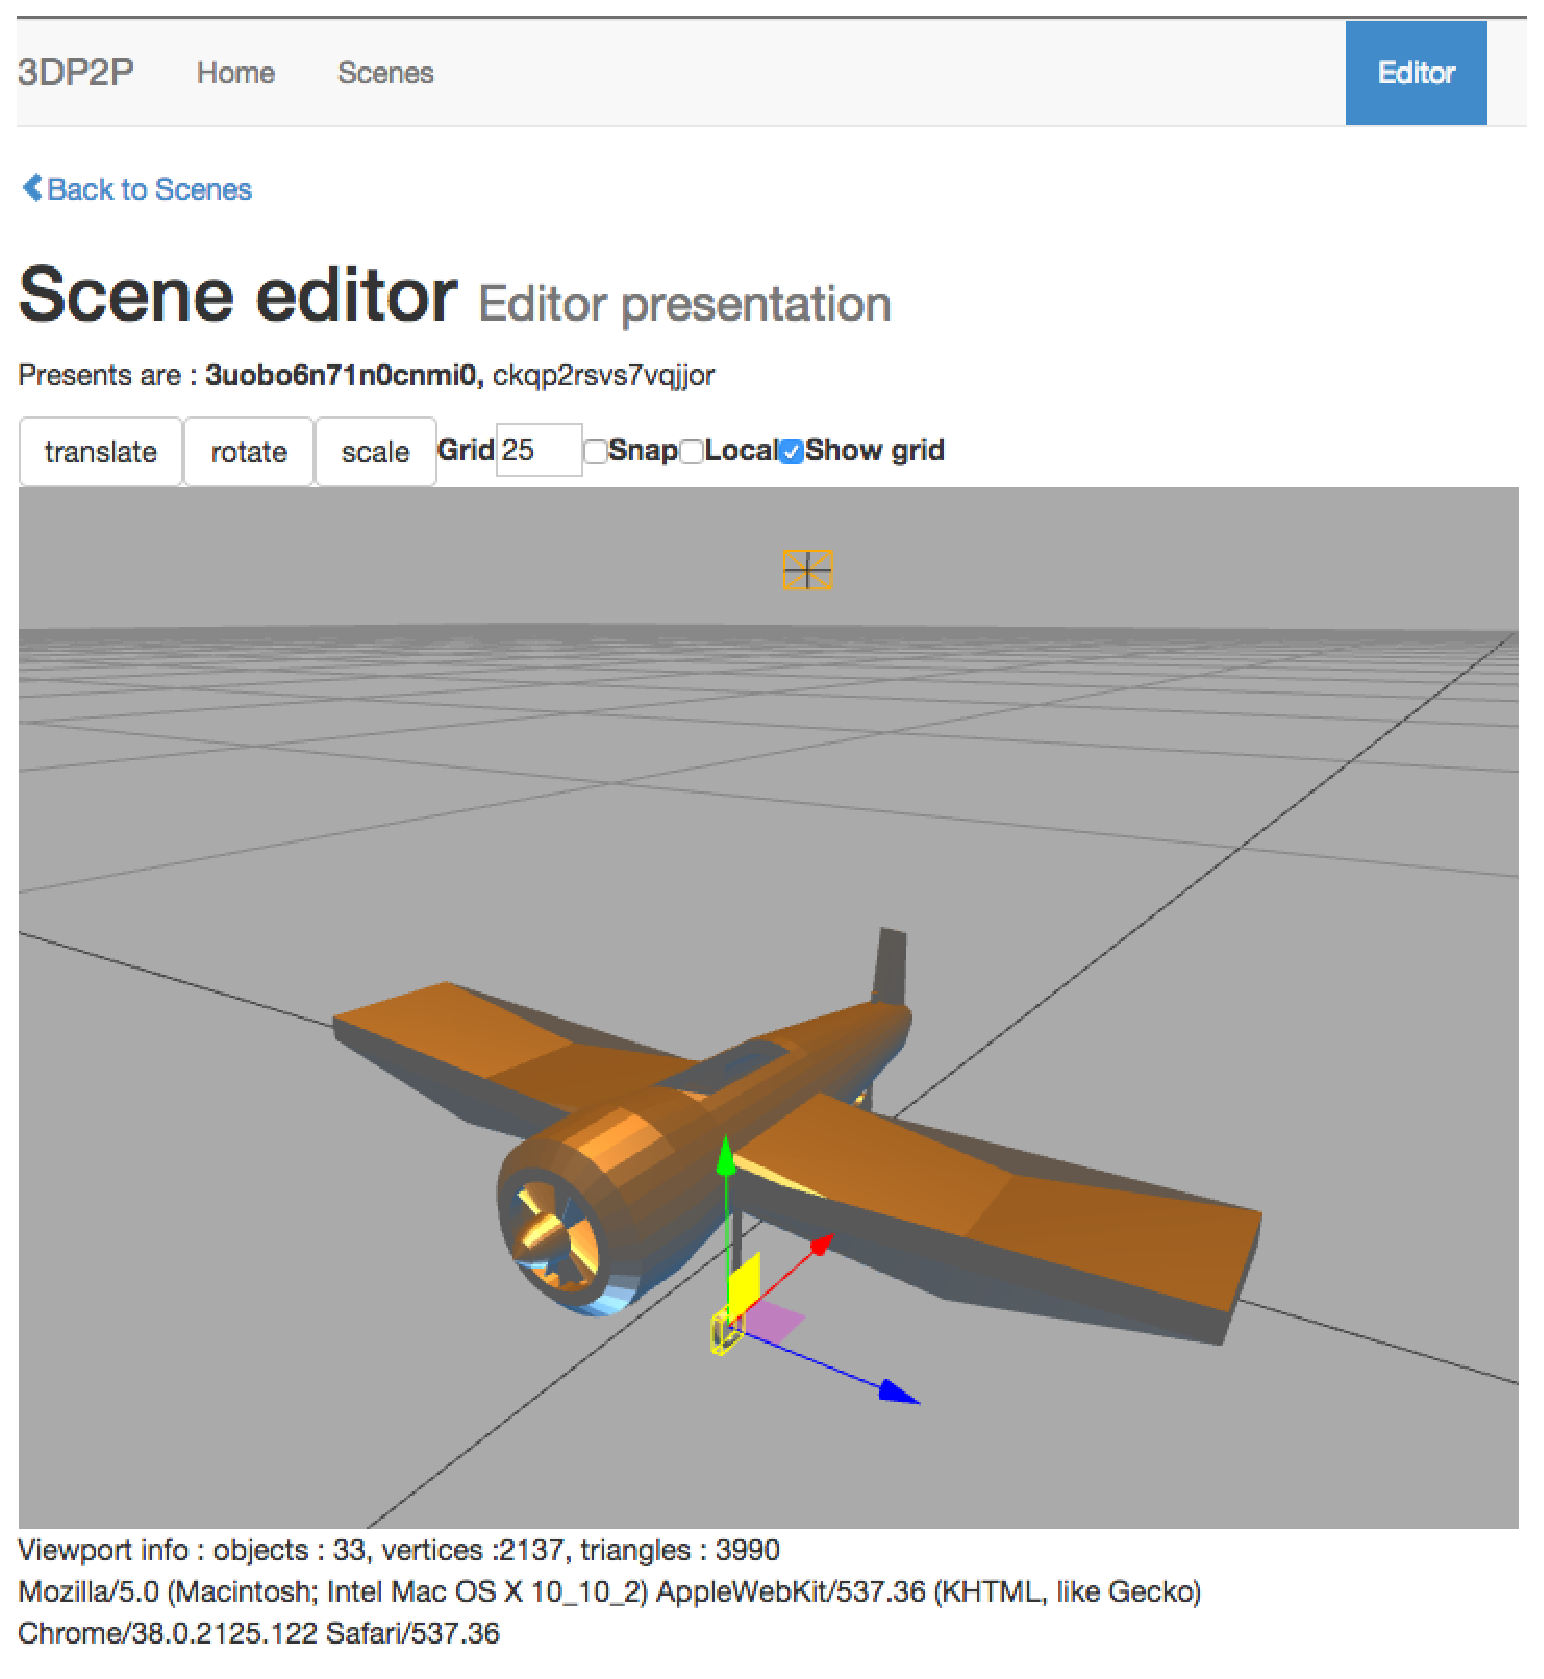
\includegraphics[width=0.6\columnwidth]{eps/editorpresentation.eps}
	\caption{Interface de 3DState}
	\label{fig:3Dstateinterface}
\end{figure}

\subsection{Gestion de la session}
Lorsqu'un utilisateur rejoint une session, il suit le déroulement des opérations 
décrit dans la Figure \ref{fig:sequence_state}. 
Dans un premier temps, afin de récupérer les données liées à l'espace de travail, 
le client web de l'utilisateur qui se rend sur une scène récupère 
tous les objets associés à la scène dans la base de données. Les objets de la 
scène sont renvoyés à l'éditeur pour les afficher. 
Dans un second temps, le système établit les connexions \gls{P2P} entre les 
clients de manière automatique et complète (topologie réseau en maillage 
complet) après avoir récupéré les identifiants des autres utilisateurs auprès du 
serveur de \textit{signaling}. Une fois la connexion établie, chaque collaborateur 
voit son environnement \gls{3D} dans l'éditeur mis à jour, indiquant la position du 
nouvel 
arrivant. Les collaborateurs éditent ensuite la scène \gls{3D} qui produit, sur les 
différents objets, des requêtes \gls{CRUD} -- incluant les opérations de translation, 
rotation et homothétie -- destinées au serveur (qui transmet les 
modifications à la base de données) puis aux collaborateurs.
Enfin, dans un dernier temps, lorsque l'utilisateur quitte la scène, il en notifie le 
serveur de \textit{signaling} qui s'occupe d'indiquer aux clients restants l'abandon 
du client pour qu'ils puissent mettre à jour leur interface en conséquence.

\begin{figure}[ht!]
	\centering
	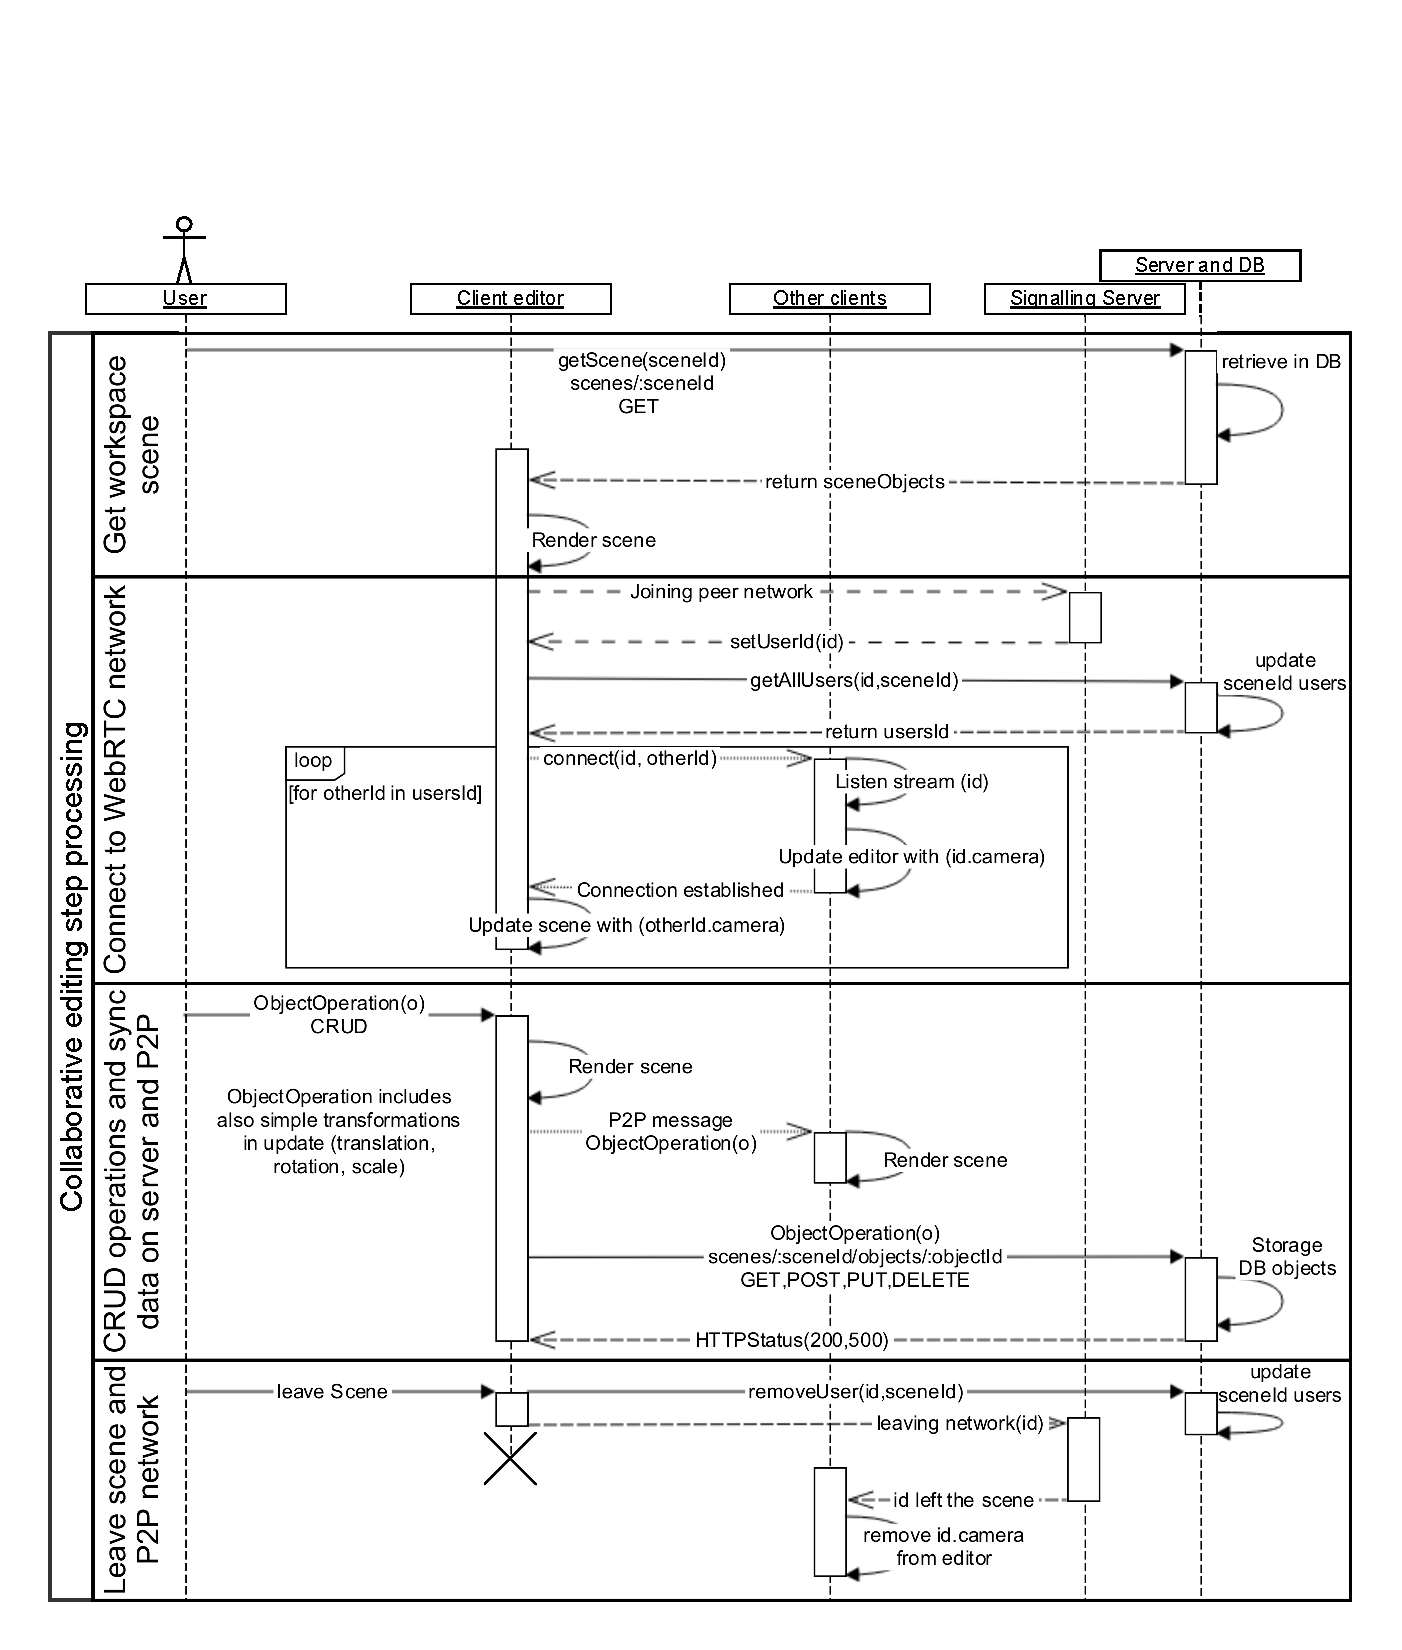
\includegraphics[trim={0 0 0 3cm},clip,width=1\columnwidth]
	{eps/sequence_wscg.eps}
	\caption{Diagramme de séquence de la gestion de la session dans une 
		architecture \og orientée état\fg{}}
	\label{fig:sequence_state}
\end{figure}

		
		\subsection{Bilan critique}
		
		
			\paragraph{Résumé des choix techniques}
			
			\begin{table}[!h]
				\centering
\caption{\label{table:3DStateChoixTechniques}Résumé des choix techniques pour 
3DState}
\begin{tabular}{llll}
	& \textbf{Plateforme / Service}& \textbf{Bibliothèque (version)}\\ \hline
	& \begin{tabular}[c]{@{}l@{}}
		Rendu WebGL \\ 
		Gestionnaire d'événements 
	\end{tabular} 	& 
	\begin{tabular}[c]{@{}l@{}}
		Three.JS (r69) \\ 
		signal-js (v1.0.0)
	\end{tabular}\\
	\multirow{-3}{*}{\textbf{Pair}} & WebRTC & PeerJS (v0.3.9)\\ \hline
	& Node.JS (v0.10.32)& ExpressJS (v4.9.0)\\
	& WebSocket & PeerJSServer (N/A) \\
	\multirow{-3}{*}{\textbf{Serveur}} & Base de données NoSQL & MongoDB 
	(v2.6.8) \\ \hline
\end{tabular}
\end{table}
			
			\paragraph{Testabilité}

\section{3DEvent : une approche découplée orientée événements}
\subsection{Intergiciel pour l'échange de 3D par événements}
\subsubsection{Données d'échanges}
\subsubsection{Synchronisation des données}
\subsubsection{Gestion de la cohérence}

\subsection{Interface orientée tâche}
Dans le but de proposer une \gls{IU} proche des fonctionnalités métiers liées à la 
modélisation \gls{3D}, l'éditeur possède une interface orientée \og tâche\fg{}, en 
comparaison avec des \gls{IU} \gls{CRUD}. En effet, les \gls{IU} \gls{CRUD} 
réduisent la sémantique métier du domaine d'application à la création, la lecture, la 
mise à jour et la suppression, omettant toutes les subtilités que peuvent dégager 
ces actions en perdant l'intention de l'utilisateur dès le niveau de l'interface. Une 
interface orientée tâche a tendance à s'attarder sur toutes les nuances que le 
domaine possède en caractérisant chaque action sans subir d'effet de 
simplification. Cette proximité avec le métier permet de calquer directement 
l'interface du modèle événementiel sur l'\gls{IU} et de guider l'utilisateur dans ses 
activités. L'utilisabilité, qualité de l'expérience utilisateur fournit par un système 
pour réaliser une tâche, est alors maximisée en terme d'efficacité, d'efficience et 
de satisfaction. 
Ce type d'\gls{IHM} s'organise autour de cas d'utilisation. Cela permet, 
d'une part, de présenter clairement les 
actions (\og ajouter une géométrie à la 
bibliothèque à partir d'un fichier\fg{} plutôt que \og téléverser un fichier\fg{}) : 
l'intention est clairement définie. D'autre part, lorsque l'utilisateur s'apprête à faire 
une action, seules les informations utiles sont affichées. Enfin, l'application fournit 
simplement l'information dans le contexte où elle doit être présentée, évitant à 
l'utilisateur d'aller la chercher ailleurs.
L'\gls{IU} devient alors une couche de l'application qui nécessite d'agréger, croiser 
et filtrer des données. La dénormalisation proposée par \gls{CQRS} remédie à ce 
besoin dans le cadre de la consultation de données. 


\subsubsection{Présentation de l'interface}


%\begin{figure}[h!]
%	\centering
%	\begingroup
%	
%	\subfloat[Rotation (vue \gls{3D}) et outils de manipulation d'objet 
%	\gls{3D} 
%	(panneau 
%	
%latéral)]{\includegraphics[width=0.75\textwidth]{eps/2rotatedetail.eps}\label{fig:ui2}}\hfill
%	
%	\subfloat[Translation (vue \gls{3D}) et visualisation de l'historique 
%	(panneau 
%	
%latéral)]{\includegraphics[width=0.75\textwidth]{eps/1translatehisto.eps}\label{fig:ui1}}\hfill
%	
%	\subfloat[Mise à l'échelle (vue \gls{3D}) et liste des collaborateurs 
%	(panneau 
%	
%latéral)]{\includegraphics[width=0.75\textwidth]{eps/3scalecollab.eps}\label{fig:ui3}}\hfill
%	
%	\endgroup
%	\caption{Interface utilisateur pendant une session collaborative (trois 
%personnes)}
%	\label{fig:screenshots}
%\end{figure}
Lorsqu'un utilisateur se connecte à une scène, il a accès à une interface web 
(dans un navigateur) qui représente l'espace de travail collaboratif et qui lui 
permettant 
d'utiliser différentes fonctionnalités. Les deux modalités d'interaction sont le clavier 
et la souris\info{est ce qu'on parle de mobile?}. Le premier niveau de cette 
interface est scindée en deux panneaux~: 
\begin{enumerate}
	\item L'espace \gls{3D} consacré à la visualisation des objets et à leur 
	manipulation 
	dans l'environnement \gls{3D}~;
	\item La barre d'outils qui contient trois onglets~:~
	\begin{enumerate}
		\item "Scene" contient tous les détails de la scène et des maillages qu'elle 
		inclue~; 
		\item "Collaboration" fournit les informations liées à la collaboration~;
		\item "History" liste tous les événements qui ont eut lieu dans la scène et 
		leurs  détails. 
	\end{enumerate}
\end{enumerate}

\begin{figure}[ht]
	\centering
	\begingroup
	
	\subfloat[Onglet \og outils de manipulation sur la 
	scène\fg{}]{\includegraphics[width=0.38\textwidth]{eps/scenecontrol.eps}\label{fig:uicontrol}}
	\hfill
	\subfloat[Onglet \og collaboration\fg{}]
	{\includegraphics[width=0.27\textwidth]{eps/collaboration.eps}\label{fig:uicollab}} 
	\hfill
	\subfloat[Onglet \og 
	historique\fg{}]{\includegraphics[width=0.32\textwidth]{eps/history.eps}\label{fig:uihisotry}}
	
	\endgroup
	\caption{Onglets du panneau latéral de l'interface}
	\label{fig:uipanneau}
\end{figure}
La Figure \ref{fig:uipanneau} montre quelques captures d'écran durant une 
session collaborative sur le modèle Rotor.

L'onglet "Scene" (Figure \ref{fig:uicontrol}) possède un bloc contenant les détails 
d'un 
maillage en cours de 
sélection. Cela permet d'avoir la description des propriétés de l'objet sélectionné et 
une manipulation de ses paramètres (position, rotation et mise à l'échelle) plus 
précise que via l'espace \gls{3D} avec le cliqué / déplacé. "Scene" intègre 
également un espace réservé aux géométries disponibles dans la scène appelé 
Bibliothèque (de géométries).

L'onglet "Collaboration" (Figure \ref{fig:uicollab}) présente la liste des 
collaborateurs qui 
participent à la 
scène. Chacun d'eux est décrit par son nom, son état  (connecté ou déconnecté) 
et son rôle (administrateur, éditeur, lecteur ou autre\footnote{Un rôle peut être 
	défini par le biais du \gls{framework} 3DEvent}). En cliquant sur un élément de 
	la 
liste, l'utilisateur accède au dernier point de vue dans l'espace \gls{3D} connu du 
collaborateur représenté.

L'onglet "History" (Figure \ref{fig:uihisotry}) liste tous les événements passés dans 
la 
scène en fournissant 
l'accès à leur détail. Pour chaque événement, le système est capable de montrer 
dans l'espace \gls{3D} la différence entre l'état  après l'événement cliqué $state_x$ 
et l'état courant $state_n$. L'utilisateur peut à partir de cette visualisation choisir 
de \og revenir en arrière\fg{} sans perdre les données entre $state_n$ et $state_x$ 
car dans le système présenté ici, cela s'effectue par compensation (cf 
Event-Sourcing 
Section X)\improve{annulation d'un événement ou juste ES}.

Dans chaque onglet se trouvent différents blocs \gls{HTML}, avec des 
comportements spécifiques à un agrégat et injectés dynamiquement. Ces blocs 
correspondent aux views de ce modèle.

Les boîtes englobantes représentent la sélection des différents collaborateurs 
pendant la session.

Parmi les views disponibles dans le système, une grande partie est dédiée à 
l'\gls{IU} de l'application web pour le cas d'utilisation de la modélisation 3D. 
D'autres views sont disponibles pour un autre type d'utilisation destinée à 
l'observation des comportements des utilisateurs, élément est primordiale dans 
une expérimentations.



\paragraph{Exemple d'interaction}
La Figure \ref{fig:cqrs-example} décrit la façon dont le système traite l'exécution 
d'une commande de translation déclenchée par l'utilisateur et comment cette 
information est diffusée aux collaborateurs\footnote{Pour que l'exemple 
	fonctionne, la scène, la géométrie du cube et le maillage \textit{cube1} doivent 
	avoir été créés en amont.}.
Dans l'étape (a), la commande déclenchée par l'utilisateur s'adresse à l'agrégat 
$cube1$ et contient les paramètres de la translation (vecteur x, y, z). L'agrégat, 
qui 
modélise le domaine d'un maillage, génère l'événement de translation $e1$ (étape 
(b)) si tout est valide d'un point de vue métier. L'événement $e1$ est ensuite 
passé à l'Event Store. 
Le composant responsable de la détection de conflit permet au développeur 
d'implémenter ses propres règles de résolution de conflit. Le composant déclenche 
une exception lorsque le numéro de version reçu et le numéro de version courant 
de l'agrégat sont identiques (Figure \ref{fig:cqrs-example} étape (c)). Selon les 
règles métiers définies et les exceptions liées à la cohérence, l'événement peut 
être 
rejeté. Ce traitement peut être à l'origine de la génération de nouveaux 
événements.


\begin{figure}[]
	\centering
	\includegraphics[width=\columnwidth]{eps/example10.eps}
	\caption[Flux de la collaboration dans le framework 3DEvent entre 3 
	utilisateurs]{Exemple d'édition collaborative où User A est connecté à User  B, 
		lui 
		même connecté à User C. Le cycle montre les différentes étapes du 
		déclenchement: la commande, la 
		génération 
		de l'événement, la 
		synchronisation du journal d'événements, l'impact sur le rendu des autres 
		utilisateurs pour une translation sur un cube et le rendu 
		visuel.}\label{fig:cqrs-example}
\end{figure}

\subsection{Sélection fantôme}
Les interactions utilisateurs doivent être adaptées à la collaboration et aux 
manipulations à effectuer. Pour cela, l'éditeur 3DEvent introduit la fonctionnalité de 
sélection \og fantôme\fg{}. Lorsqu'un utilisateur souhaite sélectionner un objet de 
la scène, l'objet original ($O_o$) est 
cloné et devient l'objet fantôme ($O_f$). $O_f$ conservent les mêmes propriétés, 
représenté avec de la 
transparence d'où le terme \og fantôme\fg{}. 
L'objet $O_f$ prend alors le focus de sélection pour que l'utilisateur le manipule à 
la place de l'objet $O_f$. 
Lorsque l'utilisateur relâche $O_f$, alors la modification intentée s'applique sur 
$O_o$ avec le principe du \textit{Last Write Wins} (le dernier gagne).
La Figure \ref{fig:ghostselection} 
représente la sélection fantôme lors de la translation du corps du rotor par 
l'utilisateur Foo : c'est l'objet transparent qui est manipulé alors que l'objet opaque 
représente sa position originale. 
En différenciant l'actuel objet que l'utilisateur souhaite sélectionné ($O_{o}$) de 
celui manipulé ($O_f$), l'interaction est mise en valeur sous quatre angles :
\begin{itemize}
	\item l'ergonomie dans l'environnement \gls{3D} :
	$O_f$ est un objet temporaire qui permet à l'utilisateur
	d'avoir une visualisation de l'objet en cours de manipulation tout en 
	conservant le dernier état de $O_o$ visible. 
	$O_o$ peut être considéré comme un point de repère visuel pour l'utilisateur 
	lorsqu'il effectue sa manipulation. 
	L'$O_f$ a aussi un rôle d'intermédiaire entre l'utilisateur et la 
	finalité de l'interaction en donnant un support visuel à sa réflexion experte.
	Grâce à $O_f$, l'utilisateur peut également révoquer sa manipulation en 
	cours sans avoir eu d'impact sur $O_o$ en évitant des actions inutiles (faire 
	l'action 
	puis la défaire) pour le métier et coûteuses pour le réseau.
	
	\item la collaboration : si un collaborateur effectue une modification 
	à destination du même $O_o$ alors la représentation de $O_o$ chez 
	l'utilisateur est également modifiée. $O_f$ par contre ne subit pas d'impact ; 
	l'utilisateur peut continuer sa manipulation et~/~ou l'ajuster en fonction des 
	nouvelles informations liées à $O_o$ ou même révoquer sa manipulation 
	en cours si cela lui convient.
	
	\item le métier : seules les manipulations menées à terme sont 
	considérées comme des commandes. Cela évite d'avoir des événements qui ne 
	sont pas pertinents pour le métier dans le journal d'événements (comme lorsque 
	l'utilisateur change d'idée lors de l'interaction ou
	suite à une intervention concurrente). L'utilisateur n'a un impact sur l'application 
	que lorsqu'une modification métier est réalisée.
	
	\item le réseau : l'information importante à faire transité est l'événement 
	correspondant à la modification métier pas toutes les positions intermédiaires 
	même si intuitivement l'idée de temps réel pourrait conduire à cette solution. La 
	quantité de messages produite surchargerai à la fois le réseau et le fil 
	d'exécution principale de l'application. En effet, \gls{WebRTC} a l'inconvénient 
	pour le 
	moment de ne pas pouvoir s'exécuter dans un \textit{Web Worker} (fil 
	d'exécution 
	parallèle en JavaScript). Cette solution imposerai des 
	latences réseau et d'\gls{IU} qui affecteraient gravement l'expérience utilisateur
	sans apporter d'informations supplémentaires à l'aspect métier de la 
	collaboration. 
\end{itemize}


\begin{figure}[ht]
	\centering
	\includegraphics[trim={0 0 0cm 0}, clip, 
	width=0.8\columnwidth]{eps/1translatehisto.eps}
	\caption{Illustration de la sélection fantôme dans l'environnement 3D}
	\label{fig:ghostselection}
\end{figure}


\subsection{Bilan}
\paragraph{Testabilité}